% Full DSDP corrupted-Alice IND-CPA secrecy auto-derivation chain.
% Each node carries \rocq{<full declaration name>} (link to the formal artifact),
% \rocqok (formalized), and \uses{...} (dependency edges).  Module prefixes:
%   infotheo.dumas2017dual.dsdp.symbolic_game.dsdp_symbolic_exec
%   infotheo.dumas2017dual.dsdp.symbolic_game.dsdp_game_derivation
%   infotheo.dumas2017dual.dsdp.symbolic_game.dsdp_game_code
%   infotheo.dumas2017dual.dsdp.indcpa_hopping.dsdp_indcpa_advantage
%   infotheo.homomorphic_encryption.indcpa_ror

\chapter{Introduction}

DSDP is a three-party scalar-product protocol built on additively homomorphic
encryption. This blueprint presents its corrupted-Alice secrecy. Alice's view
leaks through two channels, and the blueprint bounds each and composes them. The
ciphertexts she receives leak computationally, bounded by $2\,\epscpa$ from the
scheme's IND-CPA assumption. The scalar-product output $S$ she decrypts leaks
information-theoretically, bounded by $1/m$ from a fiber-counting argument that
no assumption can improve. Both bounds read off one corrupted view, and that
view is derived from the one protocol program that already defines the
protocol's behaviour, rather than written by hand. The full bound is
$1/m + 2\,\epscpa$.

The two channels split the blueprint into two parts. Part~I derives the game
from the program and bounds the ciphertext channel by $2\,\epscpa$, every choice
the argument depends on gathered in one record from which a generic theorem
reads off the advantage. It is the worked instance of the derivation framework
developed in the thesis part on the derived game. Part~II continues the same
derivation to the decryption Alice performs, exposing $S$, and bounds the output
channel by $1/m$ by citing the information-theoretic fiber theorems through one
probability identity, then composes the two bounds.

Game hopping reduces a protocol's ciphertext privacy to a chain of IND-CPA swaps
costing $k\,\epscpa$ for $k$ hops. The method takes the chain of games as given,
and someone writes that chain once per protocol: the real game, every
intermediate game, and the oracle each hop calls. For DSDP the hand-written
chain runs to several thousand lines. The derivation here removes that
hand-writing.

The derivation rests on a single idea. The protocol's procedures are written
once over an interface that names the message carriers and the homomorphic
operations and leaves their laws open. The concrete reading fills the interface
with a real encryption scheme and recovers the protocol's existing proofs
unchanged, its correctness, its termination, and its session duality. The
symbolic reading fills the interface with a free term algebra, runs the
corrupted party's procedures, and exposes the homomorphic expressions that party
sends as ordinary data. The symbolic reading is what makes the game derivable.

The chain has two halves that meet at a reified game
(Figure~\ref{fig:bp:architecture}). The front end runs the symbolic reading and
lowers the corrupted party's whole view to a first-order game syntax, a
straight-line list of samples, cell writes, encryptions, and homomorphic
assemblies. The back end denotes that syntax into an SSProve game and bounds the
adversary's advantage with one lemma that holds for every well-formed game in the
syntax. That bound is the number of encryption hops the game contains times the
single-hop IND-CPA advantage $\epscpa$. The walk that produces the view runs to
the decryption Alice performs, so the same denoted game also exposes the
scalar-product output $S$; reading the second channel off that output is the
subject of Part~II.

\begin{figure}[t]
\centering
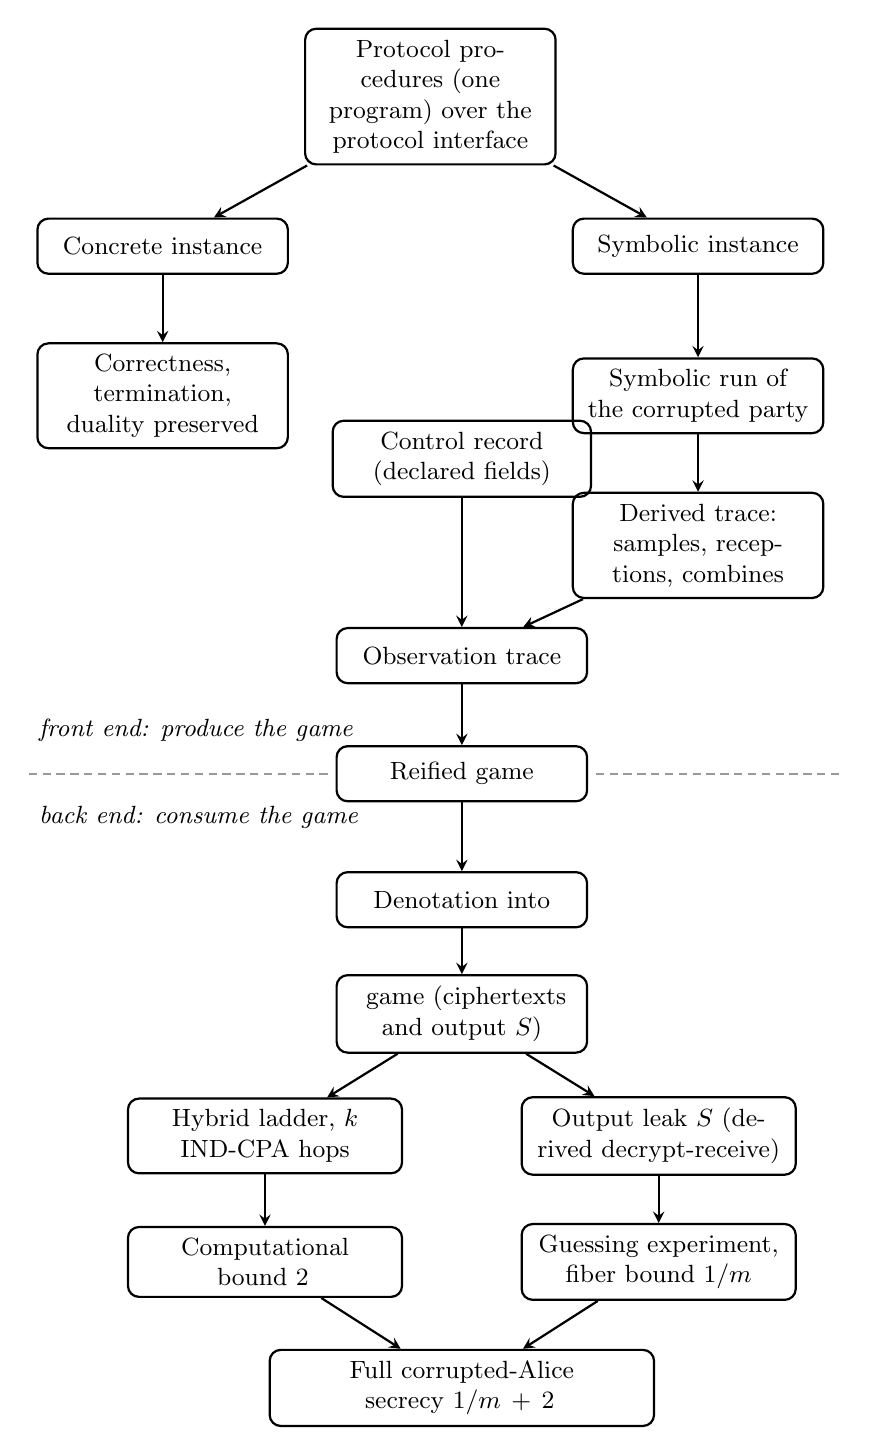
\begin{tikzpicture}[
  box/.style={draw, rounded corners, align=center, inner sep=4pt,
              font=\small, text width=2.9cm, minimum height=0.7cm},
  every path/.append style={-stealth, thick},
  font=\small
]
\node[box] (procs)  at (4,9.2)   {Protocol procedures (one program) over the protocol interface};
\node[box] (conc)   at (0.6,7.3) {Concrete instance};
\node[box] (symb)   at (7.4,7.3) {Symbolic instance};
\node[box] (proofs) at (0.6,5.4) {Correctness, termination, duality preserved};
\node[box] (run)    at (7.4,5.4) {Symbolic run of the corrupted party};
\node[box] (comb)   at (7.4,3.5) {Derived trace: samples, receptions, combines};
\node[box, text width=3.0cm] (cfg) at (4.4,4.6) {Control record (declared fields)};
\node[box] (trace)  at (4.4,2.1)  {Observation trace};
\node[box] (reif)   at (4.4,0.6)  {Reified game};
\node[box] (denote) at (4.4,-1.0) {Denotation into \ssprove{}};
\node[box] (game)   at (4.4,-2.45) {\ssprove{} game (ciphertexts and output $S$)};
\node[box, text width=3.2cm] (ladder) at (1.9,-4.0) {Hybrid ladder, $k$ IND-CPA hops};
\node[box, text width=3.2cm] (bound)  at (1.9,-5.6) {Computational bound $2\,\epscpa$};
\node[box, text width=3.2cm] (leak)   at (6.9,-4.0) {Output leak $S$ (derived decrypt-receive)};
\node[box, text width=3.2cm] (fiber)  at (6.9,-5.6) {Guessing experiment, fiber bound $1/m$};
\node[box, text width=4.6cm] (compose) at (4.4,-7.2) {Full corrupted-Alice secrecy $1/m + 2\,\epscpa$};

\draw (procs) -- (conc);
\draw (procs) -- (symb);
\draw (conc)  -- (proofs);
\draw (symb)  -- (run);
\draw (run)   -- (comb);
\draw (comb)  -- (trace);
\draw (cfg)   -- (trace);
\draw (trace) -- (reif);
\draw (reif)   -- (denote);
\draw (denote) -- (game);
\draw (game)   -- (ladder);
\draw (ladder) -- (bound);
\draw (game)   -- (leak);
\draw (leak)   -- (fiber);
\draw (bound)  -- (compose);
\draw (fiber)  -- (compose);

\draw[densely dashed, black!40, -] (-1.1,0.6) -- (2.7,0.6);
\draw[densely dashed, black!40, -] (6.1,0.6) -- (9.2,0.6);
\node[font=\itshape\small, anchor=west] at (-1.1,1.15) {front end: produce the game};
\node[font=\itshape\small, anchor=west] at (-1.1,0.05) {back end: consume the game};
\end{tikzpicture}
\caption{The derivation in two halves, meeting at the reified game, whose back
end forks into the two leakage channels. The protocol's procedures, parameterized
over one interface, admit a concrete instance (left, recovering the existing
proofs) and a symbolic instance (right). The symbolic run yields the derived
trace, and one control record supplies the declared fields. Together they form
the observation trace, which the front end lowers to the reified game. The back
end denotes that game into \ssprove{}, exposing both the received ciphertexts and
the decrypted output $S$. The ciphertext channel (left, Part~I) is bounded
through a hybrid ladder of $k$ IND-CPA hops, generically $k\,\epscpa$ and
$2\,\epscpa$ for DSDP. The output channel (right, Part~II) is bounded by the
fiber argument $1/m$. The two compose to $1/m + 2\,\epscpa$.}
\label{fig:bp:architecture}
\end{figure}

One control record carries every choice the chain depends on. It holds the
corrupted party's program, the received hop ciphertexts, the challenge secret,
the order the viewed ciphertexts leak, and the two sample-domain sizes, together
with the concrete scheme and its marshalling into SSProve choice types. From this
one record the corrupted view, the real game, the all-zero game, and the hop
count are all projections, and a single generic theorem bounds every valid
adversary's advantage by the hop count times $\epscpa$. The DSDP instance fills
the record, its hop count computes to two, and the bound reads off as
$2\,\epscpa$.

The scope is precise. The computation and the whole observation trace are derived
from the program. The sampled scalars and randomness, the receptions read off
each ciphertext's shape, and the homomorphic combinations all come from the
symbolic run rather than from a transcription. What stays declared is small and
sits as fields of the record: which party is corrupt, the secret the game
challenges, the order the viewed ciphertexts leak, and the two cardinalities. The
generality lives in the back end, whose bound applies to whatever game the record
produces.

Each entry below links to its Rocq declaration through its Rocq button. An
entry's colour records its formalization status: green for proved declarations,
and blue dashed for declarations under construction. Part~I is green throughout.
Part~II is the construction that exposes the output $S$, transports the fiber
bound to the denoted game, and composes the two channels; its entries are blue
until built. The dependency graph draws the whole chain from the control record
to the final bound.

\part{Ciphertext privacy by derived game-hopping}

\chapter{The symbolic protocol model}

\begin{definition}[Symbolic interpretation of the protocol]
  \label{def:symbolic_interface}
  \rocq{infotheo.dumas2017dual.dsdp.symbolic_game.dsdp_symbolic_exec.Symbolic_DSDP_Interface,
       infotheo.dumas2017dual.dsdp.symbolic_game.dsdp_symbolic_exec.symbolic_data}
  \rocqok
  The protocol is expressed once over an abstract interface of homomorphic
  operations. The symbolic interpretation fills that interface with a carrier of
  homomorphic syntax trees, so running a party's program records the syntactic
  assembly it performs rather than a concrete ciphertext.
  \[ d ::= \mathsf{plain}(t) \mid \mathsf{cipher}(t) \mid \mathsf{sk}(n)
        \mid \mathsf{pk}(n) \]
\end{definition}

\begin{definition}[Corrupted party's program]
  \label{def:palice_sym}
  \rocq{infotheo.dumas2017dual.dsdp.symbolic_game.dsdp_symbolic_exec.palice_sym}
  \rocqok
  \uses{def:symbolic_interface}
  The corrupted party Alice, run at the symbolic interpretation with named
  inputs. Running it is the derivation step for the messages Alice returns. Its
  leaked scalars are $u_2,r_2,u_3,r_3$ and its mask randomness $r_{a1},r_{a2}$.
\end{definition}

\begin{definition}[Sender programs and the challenge secret]
  \label{def:sender_programs}
  \rocq{infotheo.dumas2017dual.dsdp.symbolic_game.dsdp_symbolic_exec.pbob_sym,
       infotheo.dumas2017dual.dsdp.symbolic_game.dsdp_symbolic_exec.pcharlie_sym,
       infotheo.dumas2017dual.dsdp.symbolic_game.dsdp_symbolic_exec.dsdp_v2_name}
  \rocqok
  \uses{def:symbolic_interface}
  The two honest senders at the symbolic interpretation. Each one's head message
  encrypts its own secret input. Bob's secret name is the value the game later
  challenges, so the challenge provably coincides with the first received secret.
  \[ c_2 = \Enc_{pk_B}(v_2), \quad c_3 = \Enc_{pk_C}(v_3), \quad
        \text{challenge} = v_2 \]
\end{definition}

\begin{lemma}[The assembled ciphertexts are derived]
  \label{lem:observed_combines}
  \rocq{infotheo.dumas2017dual.dsdp.symbolic_game.dsdp_symbolic_exec.dsdp_observed_combines_eq}
  \rocqok
  Running the corrupted program against placeholder receptions, the two messages
  it returns compute to the two homomorphic assemblies $a_1$ and $a_2$. These
  fall out of the program and are not written by hand.
  \[ a_1 = (u_2 \hmul c_2) \hadd \Enc_{pk_B}(r_2), \qquad
        a_2 = (u_3 \hmul c_3) \hadd \Enc_{pk_C}(r_3) \]
\end{lemma}
\begin{proof}
  \uses{def:palice_sym}
  \rocqok
  By full computation on the closed symbolic terms.
\end{proof}

\begin{definition}[Received hop ciphertexts]
  \label{def:received_hops}
  \rocq{infotheo.dumas2017dual.dsdp.symbolic_game.dsdp_symbolic_exec.dsdp_received_hop_ciphertexts,
       infotheo.dumas2017dual.dsdp.symbolic_game.dsdp_symbolic_exec.first_send}
  \rocqok
  \uses{def:sender_programs}
  The stream of ciphertexts Alice receives, taken as the senders' head messages.
  By computation it is the two structured secret-bearing ciphertexts, Bob's
  encryption of $v_2$ and Charlie's encryption of $v_3$. Supplying exactly these
  fixes where the walk over Alice's program stops.
  \[ \rho = [\, c_2, \, c_3 \,] \]
\end{definition}

\chapter{Deriving the corrupted view}

\begin{definition}[Corrupted-view observations]
  \label{def:alice_obs}
  \rocq{infotheo.dumas2017dual.dsdp.symbolic_game.dsdp_game_derivation.alice_obs}
  \rocqok
  A first-order vocabulary of the actions in a corrupted party's view: sample a
  scalar, sample randomness, write the challenge cell, receive an encrypted
  secret from a party, assemble a homomorphic combination, and leak a list of
  named ciphertexts. The reception is the only hoppable action. Part~II adds one
  further action, the output reception
  (Definition~\ref{def:alice_obs_output}).
  \[ o ::= \mathsf{smp}_v(c,x) \mid \mathsf{smp}_r(c,x) \mid \mathsf{put}(x)
        \mid \mathsf{recv}(p,s,x) \mid \mathsf{comb}(x,e) \mid \mathsf{leak}(\bar x) \]
\end{definition}

\begin{definition}[Walking the program into observations]
  \label{def:walk_obs}
  \rocq{infotheo.dumas2017dual.dsdp.symbolic_game.dsdp_game_derivation.walk_obs}
  \rocqok
  \uses{def:alice_obs}
  Walk the corrupted program against the received hop ciphertexts. At each
  reception read the sending party and the encrypted secret off the ciphertext
  shape and emit a reception bound to a fresh result name. At each send emit an
  assembly of its message. For the ciphertext channel the walk stops at the
  decrypt-reception and at termination; Part~II
  (Chapter~\ref{ch:deriving_output}) continues it across that decrypt-reception
  to expose the output. On receiving $\Enc_p(s)$ it emits $\mathsf{recv}(p,s,n)$
  and recurses at $n{+}1$.
\end{definition}

\begin{definition}[Synthesising the sample prefix]
  \label{def:collect_samples}
  \rocq{infotheo.dumas2017dual.dsdp.symbolic_game.dsdp_game_derivation.collect_samples}
  \rocqok
  \uses{def:alice_obs}
  Scan the walked observations for their free scalar and randomness names in
  first-appearance order, excluding the walk's own bound result names, and emit
  one sample action per name, tagged as a plaintext scalar or an encryption
  randomness by where the name occurs.
  \[ \samples(\tau) = [\, \mathsf{smp}_\bullet(c,x) \mid x \in \mathrm{fv}(\tau) \,]
        \ \text{in first-appearance order} \]
\end{definition}

\begin{definition}[The whole corrupted-view trace]
  \label{def:obs_of_procs}
  \rocq{infotheo.dumas2017dual.dsdp.symbolic_game.dsdp_game_derivation.obs_of_procs}
  \rocqok
  \uses{def:walk_obs,def:collect_samples}
  Assemble the full trace from the loose symbolic inputs: the synthesised sample
  prefix, the challenge-cell write, the walked body, and the final leak of the
  viewed ciphertexts in the chosen order.
  \[ \mathrm{obs}(p,\rho,ch,\ell) = \samples(w) \cat [\mathsf{put}(ch)] \cat w
        \cat [\mathsf{leak}(\ell)], \quad w = \walk(p,\rho,100) \]
\end{definition}

\begin{lemma}[The derived DSDP trace]
  \label{lem:obs_of_procs_dsdp}
  \rocq{infotheo.dumas2017dual.dsdp.symbolic_game.dsdp_game_derivation.obs_of_procs_dsdp}
  \rocqok
  For the DSDP inputs the trace computes to a fourteen-action sequence: six
  scalar samples in first-appearance order, two randomness samples, the challenge
  write, two receptions, two assemblies, and the leak.
  \[ |\tau_{\mathrm{DSDP}}| = 14:\ 8\,\mathsf{smp},\ \mathsf{put}(v_2),\
        \mathsf{recv}(B,v_2),\ \mathsf{recv}(C,v_3),\ \mathsf{comb}(a_1),\
        \mathsf{comb}(a_2),\ \mathsf{leak}(a_1,a_2,c_2,c_3) \]
\end{lemma}
\begin{proof}
  \uses{def:obs_of_procs,def:palice_sym,def:received_hops}
  \rocqok
  By full computation.
\end{proof}

\begin{definition}[The DSDP corrupted-Alice trace]
  \label{def:dsdp_alice_obs}
  \rocq{infotheo.dumas2017dual.dsdp.symbolic_game.dsdp_game_derivation.dsdp_alice_obs}
  \rocqok
  \uses{def:obs_of_procs,def:palice_sym,def:received_hops,def:sender_programs}
  The DSDP instance of the whole-trace observer, with the challenge fixed to
  Bob's secret and the leak ordering assemblies before receptions. Nothing in it
  is hand-written.
  \[ \tau_{\mathrm{DSDP}} = \mathrm{obs}(P_A, [c_2,c_3], v_2,\
        \mathrm{comb}\cat\mathrm{recv}) \]
\end{definition}

\chapter{Lowering the view to reified game code}

\begin{definition}[Reified terms and game code]
  \label{def:embedding}
  \rocq{infotheo.dumas2017dual.dsdp.symbolic_game.dsdp_game_code.he_term,
       infotheo.dumas2017dual.dsdp.symbolic_game.dsdp_game_code.game_code}
  \rocqok
  A deep embedding. Homomorphic terms cover variables, constants, encryption,
  decryption, homomorphic addition, the scalar action, and ring operations.
  Straight-line game code covers sampling, the challenge write, let-binding, the
  encryption hop, and the return. The encryption hop is the only hoppable
  statement.
  \[ t ::= x \mid k \mid \Enc(p,t,r) \mid \Dec(p,t) \mid t\hadd t \mid t\hmul t
        \mid t{+}t \mid t{-}t \mid t{\cdot}t \]
  \[ g ::= \mathsf{smp}(c,g) \mid \mathsf{put}(t,g) \mid \mathsf{let}(t,g)
        \mid \mathsf{hop}(p,t,g) \mid \mathsf{ret}(\bar t) \]
\end{definition}

\begin{definition}[Resolving names to positions]
  \label{def:resolve_term}
  \rocq{infotheo.dumas2017dual.dsdp.symbolic_game.dsdp_game_derivation.resolve_term}
  \rocqok
  \uses{def:embedding}
  Rewrite a named term into the positional form the denotation expects, replacing
  each name by its binding position. Only order survives, so the particular names
  disappear from the lowered code.
  \[ \mathsf{res}_\Gamma(x) = \mathrm{idx}(x,\Gamma_v), \qquad
        \mathsf{res}_\Gamma(\Enc(p,t,r)) =
        \Enc(p, \mathsf{res}_\Gamma(t), \mathrm{idx}(r,\Gamma_r)) \]
\end{definition}

\begin{definition}[Folding observations into game code]
  \label{def:lower_obs}
  \rocq{infotheo.dumas2017dual.dsdp.symbolic_game.dsdp_game_derivation.lower_obs}
  \rocqok
  \uses{def:resolve_term,def:alice_obs,def:embedding}
  Fold the observation trace into game code, threading the value and randomness
  name environments so each resolved term lands at the right position. A
  reception becomes an encryption hop, an assembly becomes a let-binding, and the
  leak becomes the return: $\mathsf{recv}\mapsto\mathsf{hop}$,
  $\mathsf{comb}\mapsto\mathsf{let}$, $\mathsf{leak}\mapsto\mathsf{ret}$.
\end{definition}

\begin{definition}[The lowering pass]
  \label{def:game_of_trace}
  \rocq{infotheo.dumas2017dual.dsdp.symbolic_game.dsdp_game_derivation.game_of_trace}
  \rocqok
  \uses{def:lower_obs}
  Lower a corrupted-view trace to game code, starting from empty environments.
  \[ \gtrace(\tau) = \mathrm{lower}(\varepsilon, \varepsilon, \tau) \]
\end{definition}

\begin{definition}[Hop counts]
  \label{def:count_hops}
  \rocq{infotheo.dumas2017dual.dsdp.symbolic_game.dsdp_game_derivation.count_obs_hops,
       infotheo.dumas2017dual.dsdp.symbolic_game.dsdp_game_code.count_hops,
       infotheo.dumas2017dual.dsdp.symbolic_game.dsdp_game_code.hop_sites}
  \rocqok
  \uses{def:alice_obs,def:embedding}
  Two counts: the number of hoppable receptions before the leak that ends a
  trace, and the number of encryption hops in a piece of game code together with
  the list of their site indices.
  \[ \nhops(\tau) = \#\{\mathsf{recv}\text{ before }\mathsf{leak}\}, \qquad
        \sites(g) = [\, 0, \nhops(g) \,) \]
\end{definition}

\begin{lemma}[Hop-count adequacy]
  \label{lem:count_hops_adequacy}
  \rocq{infotheo.dumas2017dual.dsdp.symbolic_game.dsdp_game_derivation.count_hops_game_of_trace}
  \rocqok
  Lowering neither creates nor drops hops, so the game-side hop count of a
  lowered trace equals its protocol-side count. This ties the ladder length to
  the protocol structure.
  \[ \nhops(\gtrace(\tau)) = \nhops(\tau) \]
\end{lemma}
\begin{proof}
  \uses{def:game_of_trace,def:count_hops}
  \rocqok
  By induction over the trace, generalised over the name environments.
\end{proof}

\chapter{Denotation into SSProve}

\begin{definition}[Denotation into a package]
  \label{def:denote_game}
  \rocq{infotheo.dumas2017dual.dsdp.symbolic_game.dsdp_game_code.denote_he,
       infotheo.dumas2017dual.dsdp.symbolic_game.dsdp_game_code.denote_run,
       infotheo.dumas2017dual.dsdp.symbolic_game.dsdp_game_code.denote_game}
  \rocqok
  \uses{def:embedding}
  Evaluate game code into an SSProve package: draw each sample, write the
  challenge cell, evaluate each homomorphic term against the concrete scheme, and
  draw each encryption hop's randomness inline so it couples one-to-one with the
  IND-CPA oracle's internal sample.
  \[ \sem{\cdot} : \text{game code} \longrightarrow \text{SSProve package},
        \qquad \sem{t}_e\ \text{evaluates } t \text{ in environment } e \]
\end{definition}

\begin{definition}[Hybrid endpoints]
  \label{def:hybrid_endpoints}
  \rocq{infotheo.dumas2017dual.dsdp.symbolic_game.dsdp_game_code.zero_hop_prefix,
       infotheo.dumas2017dual.dsdp.symbolic_game.dsdp_game_code.all_real,
       infotheo.dumas2017dual.dsdp.symbolic_game.dsdp_game_code.all_zero}
  \rocqok
  \uses{def:embedding,def:count_hops}
  Replacing the secret of the first $i$ encryption hops by the canonical zero
  gives a family of games. The real game keeps every secret, and the all-zero
  game replaces all of them. Adjacent members differ at one hop.
  \[ g^{(0)} = \text{all-real}, \qquad g^{(\nhops(g))} = \text{all-zero}, \qquad
        g^{(i)}\ \text{zeroes the first } i \text{ hops} \]
\end{definition}

\chapter{The IND-CPA hybrid bound}

\begin{definition}[Single-hop IND-CPA bound]
  \label{def:indcpa_assumption}
  \rocq{infotheo.homomorphic_encryption.indcpa_ror.epsilon_cpa,
       infotheo.homomorphic_encryption.indcpa_ror.enc_ind_cpa_real_or_zero}
  \rocqok
  The scheme's assumed IND-CPA real-or-zero advantage. Any adversary's advantage
  between the real-encryption oracle and the zero-encryption oracle is at most
  $\epscpa$. This is the one cryptographic assumption the chain rests on.
  \[ \AdvE(\Oreal, \Ozero, A) \le \epscpa \]
\end{definition}

\begin{definition}[One-hop oracle routing]
  \label{def:denote_game_shim}
  \rocq{infotheo.dumas2017dual.dsdp.symbolic_game.dsdp_game_code.denote_game_shim}
  \rocqok
  \uses{def:denote_game,def:indcpa_assumption}
  Route exactly one encryption hop through the IND-CPA encryption oracle, leaving
  every other statement identical to the direct denotation. Composing it with the
  real or zero oracle reproduces one rung of the ladder. Write $\mathrm{shim}_i(g)$
  for the shim that routes hop $i$ through the oracle and inlines the rest.
\end{definition}

\begin{lemma}[Per-hop perfect equivalence]
  \label{lem:hop_equiv}
  \rocq{infotheo.dumas2017dual.dsdp.symbolic_game.dsdp_game_code.hop_equiv_real,
       infotheo.dumas2017dual.dsdp.symbolic_game.dsdp_game_code.hop_equiv_zero}
  \rocqok
  Each ladder rung equals the one-hop shim composed with the matching real or
  zero oracle, the encode-and-decode round trip at the hop collapsing.
  \[ \sem{g^{(i)}} \approx \mathrm{shim}_i(g) \circ \mathcal{O}_b, \qquad
        b \in \{\real, \zero\} \]
\end{lemma}
\begin{proof}
  \uses{def:denote_game_shim}
  \rocqok
  By structural induction on the game code, collapsing the round trip with the
  marshalling cancellations.
\end{proof}

\begin{lemma}[Adjacent rungs cost one query]
  \label{lem:advantage_hop}
  \rocq{infotheo.dumas2017dual.dsdp.symbolic_game.dsdp_game_code.advantage_hop}
  \rocqok
  Two adjacent rungs of the ladder differ at a single hop, so their advantage is
  at most the single-hop IND-CPA bound $\epscpa$.
  \[ \AdvE(\sem{g^{(i)}}, \sem{g^{(i+1)}}, A) \le \epscpa \]
\end{lemma}
\begin{proof}
  \uses{lem:hop_equiv,def:indcpa_assumption,def:hybrid_endpoints}
  \rocqok
  By a triangle chain through the two shim compositions, then the IND-CPA bound.
\end{proof}

\begin{definition}[The hybrid ladder]
  \label{def:hybrid_ladder}
  \rocq{infotheo.dumas2017dual.dsdp.symbolic_game.dsdp_game_code.hybrid_ladder}
  \rocqok
  \uses{def:denote_game,def:hybrid_endpoints}
  The intermediate rungs between the real game and the all-zero game.
  \[ \mathrm{ladder}(g) = [\, \sem{g^{(1)}}, \dots, \sem{g^{(\nhops(g)-1)}} \,] \]
\end{definition}

\begin{lemma}[Telescoping bound]
  \label{lem:advantage_sum_ladder_le}
  \rocq{infotheo.dumas2017dual.dsdp.symbolic_game.dsdp_game_code.advantage_sum_ladder_le}
  \rocqok
  A contiguous block of rungs costs at most one IND-CPA query per rung.
  \[ \text{a block of } n{+}1 \text{ rungs} \ \le\ (n{+}1)\,\epscpa \]
\end{lemma}
\begin{proof}
  \uses{lem:advantage_hop,def:hybrid_ladder}
  \rocqok
  By induction on the rung count, splitting one rung off and folding the tail.
\end{proof}

\begin{theorem}[Generic hybrid bound]
  \label{thm:advantage_le}
  \rocq{infotheo.dumas2017dual.dsdp.symbolic_game.dsdp_game_code.advantage_le}
  \rocqok
  For any game code, every valid adversary's advantage between the real and
  all-zero denoted games is at most the number of encryption hops times
  $\epscpa$.
  \[ \AdvE(\sem{g^{(0)}},\sem{g^{(\nhops(g))}},A) \ \le\ |\sites(g)|\,\epscpa \]
\end{theorem}
\begin{proof}
  \uses{lem:advantage_sum_ladder_le,def:hybrid_endpoints,def:denote_game}
  \rocqok
  A triangle chain inserts the ladder rungs; the empty ladder collapses to a
  self-advantage of zero, and the non-empty ladder telescopes through the
  contiguous-block bound.
\end{proof}

\chapter{The control record and the generic theorem}

\begin{definition}[The secrecy-problem record]
  \label{def:secrecy_problem}
  \rocq{infotheo.dumas2017dual.dsdp.symbolic_game.dsdp_game_derivation.dsdp_indcpa_secrecy_problem}
  \rocqok
  \uses{def:obs_of_procs}
  One record bundling the symbolic corrupted-view model, the corrupted program,
  the received hop ciphertexts, the challenge secret, the leak order, and the two
  sample-domain sizes, together with the concrete scheme and its marshalling into
  SSProve choice types. One value of this record determines the real game, the
  all-zero game, and the hop count.
  \[ P = (\, p, \rho, ch, \ell, c_m, c_r \,;\ E,\ \text{marshalling} \,) \]
\end{definition}

\begin{definition}[Corrupted view of a problem]
  \label{def:corrupted_view}
  \rocq{infotheo.dumas2017dual.dsdp.symbolic_game.dsdp_game_derivation.corrupted_view}
  \rocqok
  \uses{def:obs_of_procs,def:secrecy_problem}
  Apply the whole-trace observer to the record's symbolic fields.
  \[ \view(P) = \mathrm{obs}(P.p,\, P.\rho,\, P.ch,\, P.\ell) \]
\end{definition}

\begin{definition}[Real and all-zero games of a problem]
  \label{def:games}
  \rocq{infotheo.dumas2017dual.dsdp.symbolic_game.dsdp_game_derivation.game_of_problem,
       infotheo.dumas2017dual.dsdp.symbolic_game.dsdp_game_derivation.real_game,
       infotheo.dumas2017dual.dsdp.symbolic_game.dsdp_game_derivation.zero_game}
  \rocqok
  \uses{def:denote_game,def:corrupted_view,def:hybrid_endpoints,def:game_of_trace}
  Lower the corrupted view to game code, then denote its real and all-zero
  endpoints into the record's concrete scheme.
  \[ \real(P) = \sem{g^{(0)}}_E, \qquad \zero(P) = \sem{g^{(\nhops(g))}}_E,
        \qquad g = \gtrace(\view(P)) \]
\end{definition}

\begin{definition}[Valid adversary against a problem]
  \label{def:adversary}
  \rocq{infotheo.dumas2017dual.dsdp.symbolic_game.dsdp_game_derivation.dsdp_indcpa_adversary}
  \rocqok
  \uses{def:secrecy_problem}
  A distinguisher bundled with its validity and its disjointness from the game
  state and the two oracles. Quantifying over this record quantifies over all
  valid adversaries. Such an $A$ is typed by $P$'s interface and disjoint from its
  state and oracles.
\end{definition}

\begin{theorem}[Generic corrupted-view secrecy]
  \label{thm:generic_secrecy}
  \rocq{infotheo.dumas2017dual.dsdp.symbolic_game.dsdp_game_derivation.dsdp_indcpa_secrecy}
  \rocqok
  For every secrecy-problem record and every valid adversary, the advantage
  between the real game and the all-zero game is at most the corrupted view's hop
  count times $\epscpa$.
  \[ \AdvE(\real(P), \zero(P), A) \ \le\ \nhops(\view(P))\,\epscpa \]
\end{theorem}
\begin{proof}
  \uses{thm:advantage_le,lem:count_hops_adequacy,def:corrupted_view,def:games,def:adversary}
  \rocqok
  Rewrite the protocol-side hop count as the size of the game's hop-site list
  through adequacy, then apply the generic hybrid bound, discharging validity and
  the marshalling cancellations carried as fields of the record.
\end{proof}

\chapter{The DSDP instance}

\begin{lemma}[The derived game matches the fixture]
  \label{lem:dsdp_faithful}
  \rocq{infotheo.dumas2017dual.dsdp.symbolic_game.dsdp_game_derivation.dsdp_faithful}
  \rocqok
  Lowering the DSDP corrupted-Alice trace reproduces the back-end fixture game
  code exactly, binding positions and all. The fixture is therefore derived
  rather than hand-written.
  \[ \gtrace(\tau_{\mathrm{DSDP}}) = g_{\mathrm{DSDP}} \]
\end{lemma}
\begin{proof}
  \uses{def:game_of_trace,def:dsdp_alice_obs}
  \rocqok
  By full computation.
\end{proof}

\begin{definition}[The DSDP problem instance]
  \label{def:dsdp_problem}
  \rocq{infotheo.dumas2017dual.dsdp.indcpa_hopping.dsdp_indcpa_advantage.dsdp_problem}
  \rocqok
  \uses{def:secrecy_problem,def:palice_sym,def:received_hops,def:sender_programs}
  The record at the DSDP corrupted-Alice model: the corrupted program, the
  derived hop stream, and the challenge fixed to Bob's secret, together with a
  supplied scheme and marshalling. This is the whole input a researcher provides.
  \[ P_{\mathrm{DSDP}} = (\, P_A, [c_2,c_3], v_2,\ \mathrm{comb}\cat\mathrm{recv},
        c_m, c_r \,;\ E, \dots \,) \]
\end{definition}

\begin{lemma}[Two hops]
  \label{lem:dsdp_problem_hops}
  \rocq{infotheo.dumas2017dual.dsdp.indcpa_hopping.dsdp_indcpa_advantage.dsdp_problem_hops}
  \rocqok
  The DSDP corrupted view has exactly two encryption hops, one for Bob's secret
  and one for Charlie's.
  \[ \nhops(\view(P_{\mathrm{DSDP}})) = 2 \]
\end{lemma}
\begin{proof}
  \uses{def:dsdp_problem,def:count_hops,def:corrupted_view}
  \rocqok
  By computation.
\end{proof}

\begin{theorem}[DSDP corrupted-Alice secrecy]
  \label{thm:dsdp_secure}
  \rocq{infotheo.dumas2017dual.dsdp.dsdp_main.dsdp_alice_view_advantage_le}
  \rocqok
  Every valid adversary's advantage between the real and all-zero DSDP games is
  at most $2\,\epscpa$.
  \[ \AdvE(\real(P_{\mathrm{DSDP}}), \zero(P_{\mathrm{DSDP}}), A) \ \le\
        2\,\epscpa \]
\end{theorem}
\begin{proof}
  \uses{thm:generic_secrecy,def:dsdp_problem,lem:dsdp_problem_hops}
  \rocqok
  Specialise the generic theorem to the DSDP problem and rewrite the hop count to
  two.
\end{proof}

\begin{corollary}[Loose-argument form]
  \label{cor:dsdp_advantage_derived}
  \rocq{infotheo.dumas2017dual.dsdp.indcpa_hopping.dsdp_indcpa_advantage.dsdp_advantage_derived}
  \rocqok
  The same $2\,\epscpa$ bound stated directly over the denoted games, packaging
  the loose arguments into the record.
\end{corollary}
\begin{proof}
  \uses{thm:generic_secrecy,def:dsdp_problem}
  \rocqok
  Package the loose arguments into the record and adversary, then apply the
  generic theorem.
\end{proof}

% Part II: continue the SAME derivation across Alice's decrypt-receive to expose
% the output S, build the absolute-Pr guessing layer on the DERIVED endpoint
% game, transport the Infotheo fiber 1/m through one probability identity, and
% compose with the Part I 2*epsilon_cpa.  See it_bound_bridge.tex.
\part{Output secrecy and the full bound}
% =====================================================================
% Part II: Output secrecy and the full bound.
%
% Continues the Part I derivation across Alice's decrypt-receive to expose the
% scalar-product output S, builds the absolute-Pr guessing layer on the DERIVED
% endpoint game, transports the Infotheo fiber 1/m to that game through one
% probability identity, and composes with the Part I 2*epsilon_cpa.
%
% Colour / status convention (same as content.tex):
%   \rocqok + \rocq{...}  green : ALREADY EXISTS, cited as a black box.
%   no \rocqok, no \rocq  blue  : TO CONSTRUCT (this plan).
%
% Statement bodies are terse mathematical statements (no proof, no status, no
% motivation).  Proof strategy and the exact Coq names to construct live in
% "% proof:" / "% to create:" comments for the implementer.  Identifiers are
% written in clean math (no \texttt).
%
% Existing module prefixes cited as green:
%   infotheo.dumas2017dual.dsdp.dsdp_game_symbolic   (derived view, Part I)
%   infotheo.dumas2017dual.dsdp.dsdp_indcpa_security (derived 2*epsilon_cpa)
%   infotheo.dumas2017dual.dsdp.dsdp_entropy         (fiber facts)
%   infotheo.dumas2017dual.entropy_fiber.entropy_fiber_zpq
% New identifiers land in the derived chain (dsdp_game_symbolic / dsdp_game_code
% / dsdp_indcpa_security) and a new module dsdp_security_indcpa_fiber.
%
% New notation local to Part II.
\newcommand{\fib}{\mathrm{fiber}}
\newcommand{\guess}{\mathrm{guess}}
\newcommand{\cond}{\mathrm{cond}}
\newcommand{\Prexp}{\Pr\nolimits_{\mathrm{exp}}}
% =====================================================================

\chapter{Extending the derivation to Alice's decryption}
\label{ch:deriving_output}

In the protocol Alice receives the masked aggregate, decrypts it, and removes
her masks to read the scalar-product output $S=U_1V_1+U_2V_2+U_3V_3$. The Part~I
walk stops one reception short of this decrypt
(Definition~\ref{def:walk_obs}), so the derived view exposes only the
ciphertexts. This chapter continues the same walk across that decrypt-reception,
lowers and denotes the new observation, and so the derived endpoint game exposes
$S$ alongside the ciphertexts. Adjoining $S$ to both endpoints is a common
deterministic post-processing: it adds no encryption hop, so the Part~I bound
$2\,\epscpa$ carries over unchanged.

\begin{definition}[Output reception]
  \label{def:alice_obs_output}
  \uses{def:alice_obs}
  % to create: alice_obs constructor AO_recv_output (dsdp_game_symbolic).
  The corrupted-view vocabulary (Definition~\ref{def:alice_obs}) gains one
  action: receive the decrypted output and bind it to a result name. It is not
  an encryption hop.
  \[ o \mathrel{::=} \dots \mid \mathsf{recvOut}(x) \]
\end{definition}

\begin{definition}[Walking across the decrypt-reception]
  \label{def:walk_obs_output}
  \uses{def:walk_obs,def:alice_obs_output}
  % to create: extend walk_obs (dsdp_game_symbolic) with the decrypt-receive arm
  %   and feed the three-element response stream dsdp_recv_responses (the third
  %   entry HE_var 50 is Alice's decrypt input); emit AO_recv_output carrying the
  %   he_term for S, then halt.
  At the decrypt-reception the extended walk reads the received plaintext off the
  response stream and emits the output reception instead of halting. The
  ciphertext receptions and assemblies before it are unchanged, so the
  encryption-hop count is unchanged.
\end{definition}

\begin{lemma}[The derived output-exposing DSDP trace]
  \label{lem:obs_of_procs_dsdp_leak_S}
  \uses{lem:obs_of_procs_dsdp,def:walk_obs_output}
  % to create: obs_of_procs_dsdp_leak_S, the equational characterisation of the
  %   extended obs_of_procs on the DSDP inputs; computes to the Part I trace plus
  %   one AO_recv_output before the leak.
  For the DSDP inputs the extended trace computes to the Part~I trace
  (Lemma~\ref{lem:obs_of_procs_dsdp}) with the output reception inserted before
  the leak. The two encryption hops are exactly the Part~I two.
  \[ \tau^{S}_{\mathrm{DSDP}}
        = \tau_{\mathrm{DSDP}} \text{ with } \mathsf{recvOut}(S)
        \text{ before } \mathsf{leak} \]
\end{lemma}

\begin{definition}[Lowering the output reception]
  \label{def:lower_obs_output}
  \uses{def:lower_obs,def:alice_obs_output}
  % to create: extend lower_obs (dsdp_game_symbolic) with the AO_recv_output arm
  %   -> a let binding the resolved S term followed by a put to S_output_cell;
  %   reuses existing game_code constructors (let, put), so game_code is NOT
  %   extended.
  The lowering pass maps the output reception to a let-binding of the resolved
  output term followed by a write to a dedicated output cell. It introduces no
  new game-code statement and no new hop.
  \[ \mathsf{recvOut}(S) \;\mapsto\; \mathsf{let}(S);\ \mathsf{put}_{S}(S) \]
\end{definition}

\begin{definition}[Denoting the output and exposing it]
  \label{def:denote_game_leak_S}
  \uses{def:denote_game,def:lower_obs_output}
  % to create: S_output_cell : Location; id_s_get oracle id; denote_s_get_body;
  %   widen the denoted game's export interface with #val #[id_s_get] : 'unit ->
  %   t_msg returning S_output_cell.  GC_ret stays cipher_list, so the Part I
  %   generic theorem is untouched.
  Denotation writes the lowered output to a dedicated cell and adds one oracle
  reading it, leaving the return value and every other statement as in Part~I
  (Definition~\ref{def:denote_game}).
  \[ \sem{\mathsf{put}_{S}(S)} : \text{write } S \text{ to } S\text{-cell},
        \qquad \mathsf{getOut} : \mathbf{1} \to \mathsf{msg} \]
\end{definition}

\begin{definition}[The output-exposing endpoint games]
  \label{def:games_leak_s}
  \uses{def:denote_game_leak_S,def:games}
  % to create: real_game_leak_S, zero_game_leak_S (dsdp_indcpa_security), the
  %   real/all-zero denotations of the output-exposing DSDP problem.
  The real and all-zero games of the DSDP problem
  (Definition~\ref{def:games}) denoted from the output-exposing derivation. Each
  exposes the ciphertexts and the output $S$. Write $\real_S$ and $\zero_S$ for
  the two.
  \[ \view = \big(\,[\,a_1,a_2,c_2,c_3\,],\ S\,\big),\qquad
        S = u_1 v_1 + u_2 v_2 + u_3 v_3 \]
\end{definition}

\begin{lemma}[Computational distance, output-exposing games]
  \label{lem:dsdp_advantage_derived_leak_S}
  \uses{def:games_leak_s,thm:dsdp_secure}
  % to create: dsdp_advantage_derived_leak_S; the output cell is a common
  %   deterministic post-processing of both endpoints (no new hop), so the
  %   Part I 2*epsilon_cpa bound (thm:dsdp_secure) transports verbatim.
  The advantage between the output-exposing real and all-zero games is at most
  $2\,\epscpa$, the Part~I bound (Theorem~\ref{thm:dsdp_secure}).
  \[ \AdvE(\,\real_S,\ \zero_S,\ A\,) \le 2\,\epscpa \]
\end{lemma}

\chapter{The output-secrecy guessing experiment}
\label{ch:guessing_experiment}

The output channel is measured not by an advantage but by the absolute
probability that a predictor, reading the view including $S$, names Bob's secret
$V_2$. This chapter builds that guessing experiment on the derived endpoint game
and rewrites its success probability as an Infotheo distribution probability, the
single identity that carries the fiber bound of Chapter~\ref{ch:it_bound} to the
\ssprove{} side.

\begin{definition}[Guessing experiment on the endpoint game]
  \label{def:guessing_experiment_leak_S}
  \uses{def:games_leak_s}
  % to create: predictor_guesser, guessing_challenger, guessing_experiment
  %   (dsdp_security_indcpa_fiber).  Challenger imports id_game_run, id_s_get,
  %   id_v2_get; feeds (ciphertexts, S) to the predictor; tests guess == V2.
  A predictor reads the leaked ciphertexts and the output $S$ and returns a
  guess. The experiment runs it against the endpoint game and tests
  $\guess = V_2$. Its success probability is written $\Prexp(\text{game})$.
  \[ \Prexp(\text{game})
        = \mu\big(\mathrm{Pr}(\,\text{challenger}\circ\text{predictor}
        \circ\text{game}\,)\big)(\mathrm{true}) \]
\end{definition}

\begin{lemma}[\ssprove{} absolute-$\mathrm{Pr}$ reflection calculus (library)]
  \label{lem:exist_pr_code}
  \rocqok
  % library: Pr_code_ret/_sample/_bind/_get/_put (Crypt.nominal.Pr), dlet_uniform
  %   (Crypt.HybridArgument), SDistr = {distr A/R}, dletE, dunit1E, Pr_Pr_fst.
  SSProve's nominal layer expresses the probability of a closed program as an
  iterated sum over its sample operations, a uniform draw of domain $n$
  contributing the factor $1/n$. Its subdistribution type is the
  mathcomp-analysis distribution $\{\mathrm{distr}\ A/R\}$.
  \[ \mathrm{Pr}(x \leftarrow \mathrm{sample}\ \mathrm{unif}\,n \,;;\, k\,x)
        = \tfrac1n{\textstyle\sum_x}\mathrm{Pr}(k\,x) \]
\end{lemma}

\begin{definition}[The guessing-experiment distribution]
  \label{def:dsdp_guess_fdist}
  \uses{def:guessing_experiment_leak_S}
  % to create: dsdp_guess_fdist (dsdp_security_indcpa_fiber), the uniform fdist
  %   on the experiment's sample tuple; V2,V3,U2,U3,S,guess as RVs over it.
  The uniform distribution $P$ on the samples of the guessing experiment at
  $\zero_S$, the game's draws together with the predictor's. The protocol
  quantities and the predictor's output are random variables over $P$.
  \[ P : \{\mathrm{fdist}\ \mathrm{Samples}\},
        \qquad V_2,\,V_3,\,U_2,\,U_3,\,S,\,\guess : \{\mathrm{RV}\ P\} \]
\end{definition}

\begin{lemma}[The game probability is the fdist probability]
  \label{lem:Pr_guess_enc_zero_leak_S_eqE}
  \uses{def:games_leak_s,def:dsdp_guess_fdist,def:guessing_experiment_leak_S,lem:exist_pr_code}
  % to create: Pr_guess_enc_zero_leak_S_eqE (the connector).  Proof: the closed
  %   experiment denotes to the uniform distribution on its samples, which is P
  %   (the predictor's draws are extra coordinates of P, so an opaque predictor
  %   needs no inspection); reflection (lem:exist_pr_code) rewrites both sides to
  %   the uniform average of [guess = V2].  ~30-80 lines, one induction over the
  %   sample list.
  $\Prexp(\zero_S)$ equals the Infotheo probability, over $P$, of the event
  $\guess = V_2$. Both reduce to the same uniform average of the indicator
  $[\,\guess = V_2\,]$ over the experiment's samples. This identity carries the
  fiber bound, proved on the Infotheo side, to $\Prexp(\zero_S)$.
  \[ \Prexp(\zero_S) = \Pr\nolimits_{P}[\,\guess = V_2\,] \]
\end{lemma}

\chapter{The information-theoretic bound and full secrecy}
\label{ch:it_bound}

Conditioned on $S$ and her inputs, Bob's secret $V_2$ is uniform over a fiber of
$m$ points, so any guess succeeds with probability at most $1/m$. Infotheo proves
this over an abstract joint distribution. Instantiating that distribution at the
guessing-experiment distribution $P$ and pushing the bound through the connector
(Lemma~\ref{lem:Pr_guess_enc_zero_leak_S_eqE}) gives the output bound at the
endpoint, and composing with the computational distance gives the full secrecy
bound $1/m + 2\,\epscpa$.

\section{Reused Infotheo facts}

\begin{lemma}[Fiber cardinality is $m$]
  \label{lem:exist_fiber_card}
  \rocq{infotheo.dumas2017dual.dsdp.dsdp_entropy.dsdp_fiber_card}
  \rocqok
  The solution set of the scalar-product constraint, for admissible
  multipliers, has exactly $m$ points.
  \[ \#\lvert \fib(u_1,u_2,u_3,v_1,s)\rvert = m \]
\end{lemma}

\begin{lemma}[Conditional uniformity on the fiber]
  \label{lem:exist_cpr_fiber}
  \rocq{infotheo.dumas2017dual.entropy_fiber.entropy_fiber_zpq.cPr_uniform_fiber}
  \rocqok
  \uses{lem:exist_fiber_card}
  For a joint distribution in which the variable pair is uniform and
  independent of the inputs, conditioning on the revealed values leaves the
  variable uniform over its fiber.
  \[ \Pr[\,\mathrm{Var}=v \mid \mathrm{Cond}=\cond\,]
        = \#\lvert\fib(\cond)\rvert^{-1} \]
\end{lemma}

\begin{lemma}[DSDP solution is uniform, probability $1/m$]
  \label{lem:exist_pr_sol}
  \rocq{infotheo.dumas2017dual.dsdp.dsdp_entropy.Pr_dsdp_sol_uniform}
  \rocqok
  \uses{lem:exist_cpr_fiber,lem:exist_fiber_card}
  Each solution $(v_2,v_3)$ of the DSDP constraint has conditional probability
  $1/m$ given the inputs and $S$.
  \[ \Pr[\,(V_2,V_3)=(v_2,v_3)\mid \mathrm{Cond}=\cond\,] = m^{-1} \]
\end{lemma}

\begin{theorem}[Residual entropy is $\log m$]
  \label{thm:exist_centropy}
  \rocq{infotheo.dumas2017dual.dsdp.dsdp_entropy.dsdp_centropy_uniform}
  \rocqok
  \uses{lem:exist_pr_sol}
  Conditioned on the inputs and $S$, the variable pair retains $\log m$ bits of
  entropy.
  \[ H(\mathrm{Var}\mid \mathrm{Cond}) = \log m \]
\end{theorem}

\section{Instantiating the fiber bound at $P$}

\begin{lemma}[Distribution identities: uniformity, independence, constraint]
  \label{lem:dsdp_guess_identities}
  \uses{def:dsdp_guess_fdist,def:games_leak_s}
  % to create: dsdp_guess_V2_uniform, dsdp_guess_VarRV_indep_inputs,
  %   dsdp_guess_S_determined, dsdp_guess_indep_V2_given_S
  %   (dsdp_security_indcpa_fiber); the hypotheses dsdp_entropy needs, read off
  %   the uniform structure of P and the all-zero ciphertexts.
  Over $P$, the variable pair $(V_2,V_3)$ is uniform and independent of the
  inputs, the output $S$ is the constraint function of the variables and inputs,
  and the guess depends on $V_2$ only through $S$.
  \[ {p}_{(V_2,V_3)} = \mathrm{unif},\quad
     (V_2,V_3)\perp \mathrm{Inputs},\quad
     S = g(\mathrm{Var},\mathrm{Input}),\quad
     \guess \perp V_2 \mid S \]
\end{lemma}

\begin{lemma}[Fiber residual]
  \label{lem:Pr_guess_fiber_le_invm}
  \uses{lem:exist_pr_sol,lem:dsdp_guess_identities}
  % to create: Pr_guess_fiber_le_invm (dsdp_security_indcpa_fiber).  Proof:
  %   condition on S; lem:exist_pr_sol gives each V2 value probability 1/m, and
  %   guess _|_ V2 | S (lem:dsdp_guess_identities) caps the collision at 1/m.
  Over $P$, the predictor guesses $V_2$ with probability at most $1/m$.
  \[ \Pr\nolimits_{P}[\,\guess=V_2\,] \le 1/m \]
\end{lemma}

\section{The output bound and composition}

\begin{theorem}[Information-theoretic bound at the endpoint]
  \label{thm:Pr_guess_enc_zero_leak_S_le_invm}
  \uses{lem:Pr_guess_enc_zero_leak_S_eqE,lem:Pr_guess_fiber_le_invm}
  % to create: Pr_guess_enc_zero_leak_S_le_invm (dsdp_security_indcpa_fiber).
  %   Proof: rewrite Prexp(zero_S) by the connector, then the fiber residual.
  At the output-exposing all-zero endpoint, the predictor guesses $V_2$ with
  probability at most $1/m$.
  \[ \Prexp(\zero_S) \le 1/m \]
\end{theorem}

\begin{theorem}[Full secrecy by composition]
  \label{thm:dsdp_alice_secrecy_leak_S}
  \uses{thm:Pr_guess_enc_zero_leak_S_le_invm,lem:dsdp_advantage_derived_leak_S}
  % to create: dsdp_alice_secrecy_leak_S (dsdp_security_indcpa_fiber).  Proof:
  %   triangle Prexp(real_S) <= Prexp(zero_S) + AdvE(real_S, zero_S, predictor),
  %   then thm:Pr_guess_enc_zero_leak_S_le_invm (1/m) and
  %   lem:dsdp_advantage_derived_leak_S (2*epsilon_cpa).
  Against the output-exposing real game, the predictor guesses $V_2$ with
  probability at most $1/m + 2\,\epscpa$.
  \[ \Prexp(\real_S) \le 1/m + 2\,\epscpa \]
\end{theorem}

